\documentclass{article}
\usepackage[T1]{fontenc}
\usepackage{lmodern}
\usepackage{graphicx}
\usepackage{amsmath,amssymb}
\usepackage[a4paper,margin=2cm]{geometry}
\usepackage[absolute,overlay]{textpos}
\setlength{\TPHorizModule}{1mm}
\setlength{\TPVertModule}{1mm}
\usepackage[indonesian]{babel}
\usepackage{hyperref}
\setlength{\emergencystretch}{2em}
% unit: Halaman 1

\begin{document}

% === Halaman 1 (llm) ===

\begin{center}
Bahan kuliah IF4020 Kriptografi

{\Huge \textbf{Elliptic Curve Cryptography (ECC)}} \\
{\Large (Bagian 1)}

\vspace{40mm}

\textbf{Oleh: Rinaldi Munir}

\vspace{10mm}

Program Studi Teknik Informatika \\
Sekolah Teknik Elektro dan Informatika \\
Institut Teknologi Bandung \\
2026
\end{center}

% deskripsi: Ilustrasi geometris operasi penjumlahan titik pada kurva eliptik yang menunjukkan titik P, Q, hasil penjumlahan P+Q, dan hasil perkalian P*Q.
% bbox normalisasi: [0.7420, 0.2630, 0.9570, 0.6760]
\begin{textblock*}{45.15mm}(155.82mm,78.11mm)
\noindent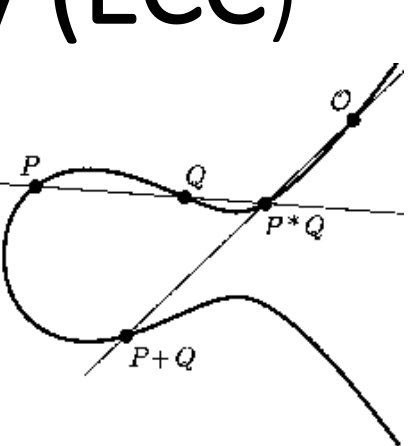
\includegraphics[width=45.15mm,height=122.66mm]{../../images/llm/page_001_img_01.png}%
\end{textblock*}

\end{document}
